\documentclass[12pt]{article}

\usepackage[margin=1.5cm]{geometry}        % For setting margins
\usepackage[spanish,es-tabla]{babel}
\selectlanguage{spanish}
\usepackage{amsmath}                % For Math
\usepackage{fancyhdr}                % For fancy header/footer
\usepackage{graphicx}                % For including figure/image
\usepackage{cancel}                    % To use the slash to cancel out stuff in working out equations
\usepackage{amsfonts}
\usepackage{color}
\usepackage{bbm}
\usepackage{float}
\usepackage{subcaption}
\usepackage{lipsum}
\usepackage{listings}
\usepackage{algorithm,algpseudocode}
\usepackage{hyperref}
\captionsetup{compatibility=false}

%%%%%%%%%%%%%%%%%%%%%%
% Set up fancy header/footer
\pagestyle{fancy}
\fancyhead[LO,L]{Alejandro Uribe}
\fancyhead[CO,C]{Aprendizaje Reforzado - Guía 1: Multi-armed bandits}
\fancyhead[RO,R]{}
\fancyfoot[LO,L]{}
\fancyfoot[CO,C]{\thepage}
\fancyfoot[RO,R]{\today}
\renewcommand{\headrulewidth}{0.4pt}
\renewcommand{\footrulewidth}{0.4pt}

\newlength\tindent
\setlength{\tindent}{\parindent}
\setlength{\parindent}{0pt}
\renewcommand{\indent}{\hspace*{\tindent}}
\DeclareMathOperator*{\argmax}{argmax}
\floatname{algorithm}{Algoritmo}
%%%%%%%%%%%%%%%%%%%%%%

\begin{document}
    \indent\underline{\textbf{Ejercicio 1}}\\
    Demostrar que, si conociéramos exactamente el valor de cada acción, es decir, si $Q_{t} (a) = E \left[ R_{t} \big| A_{t}=a \right]$, entonces la acción \textit{greedy} $ A_{t} = \argmax_{a}Q_{t}(a) $ es la acción óptima en el sentido de que permite maximizar las recompensas totales.

    \indent\underline{\textbf{Solución}}\\
    Sea,\\
    $a$: Acción arbitraria \\
    $A_{t}$: Acción tomada en el tiempo $t$ \\
    $R_{t}$: Recompensa obtenida en el tiempo $t$ \\
    $Q_{t}(a)$: Valor estimado de la acción $a$ en el tiempo $t$ \\
    $q_{*}(a)$: Recompensa esperada al tomar la acción $a$ \\
    \textit{Acción greedy}: acción que maximiza el valor esperado de la recompensa \\

    El valor $q_{*}(a)$ de una acción $a$ equivale a la recompensa esperada si se selecciona dicha acción.

    \[ q_{*}(a) \doteq \mathbb{E} \left[ R_{t} \big| A_{t}=a \right] \]

    El algoritmo \textit{greedy}, \textit{no exploratorio}, estima $Q_{t}(a)$ como el promedio de las recompensas obtenidas, es decir,

    \[
        Q_{t}(a)
        \doteq
        \frac{\text{suma de las recompensas obtenidas al seleccionar \textbf{a}}}
        {\text{número de veces que se seleccionó \textbf{a}}}
    \]

    En cada tiempo \textit{t}, el algoritmo \textit{greedy} selecciona la acción $a$ que maximiza el valor esperado de la recompensa, es decir, la acción $a$ tal que $Q_{t}(a) = q_{*}(a)$.
    En otras palabras, en cada paso, el algoritmo elige la acción que tiene la mayor recompensa esperada, matemáticamente se expresa como

    \begin{align*}
        A_{t} &= \argmax_{a}Q_{t}(a) \\
        &= \argmax_{a}q_{*}(a)
    \end{align*}

    Dado que $q_{*}(a)$ es la recompensa esperada real, al seleccionarla se obtiene la mayor recompensa posible.
    Por lo tanto, la acción \textit{greedy} $ A_{t} = \argmax_{a}Q_{t}(a) $ es la acción óptima en el sentido de que permite maximizar las recompensas totales.

    \line(1,0){\textwidth}

    \indent\underline{\textbf{Ejercicio 2}}\\
    En una selección de acciones tipo $\varepsilon-greedy$ con dos acciones posibles y $\varepsilon=0.1$, ¿Cuál es la probabilidad de seleccionar la acción \textit{greedy}?

    \indent\underline{\textbf{Solución}}\\
    En una estrategia de acciones tipo $\varepsilon-greedy$, se selecciona una acción aleatoria con probabilidad $\varepsilon$ y se selecciona la acción \textit{greedy} con probabilidad $1-\varepsilon$.
    Es decir, si $\varepsilon=0.1$, entonces la probabilidad de seleccionar la acción \textit{greedy} es de $1-\varepsilon=0.9$.
    O bien,

    \[P(\text{acción \textit{greedy}}) = 1-\varepsilon = 1 - 0.1 = 0.9\]

    Por lo tanto, la probabilidad de seleccionar la acción \textit{greedy} es $0.90$ o el $90\%$.

    \line(1,0){\textwidth}

    \indent\underline{\textbf{Ejercicio 3}}\\
    Demostrar que el valor de una acción después de haber sido seleccionada $n-1$ veces, definido como

    \[ Q_{n} = \frac{R_{1} + R_{2} + \ldots + R_{n-1}}{n-1} \]

    puede calcularse incrementalmente con la siguiente fórmula:

    \[ Q_{n+1} = Q_{n} + \frac{1}{n} \left[ R_{n} - Q_{n} \right] \]

    Describa la ventaja de esta fórmula desde un punto de vista computacional.

    \indent\underline{\textbf{Solución}}

    Sea,\\
    $Q_{n}$: Valor estimado de la acción después de haber sido seleccionada $n-1$ veces \\
    $R_i$: Recompensa obtenida después de la $i$-ésima selección de la acción \\
    $n$: Número de veces que la acción ha sido seleccionada \\

    Dado que $Q_{n}$ es el promedio de las recompensas obtenidas después de haber seleccionado la acción $n-1$ veces, se tiene que

    \[ Q_{n} = \frac{R_{1} + R_{2} + \ldots + R_{n-1}}{n-1} \]

    O bien puede escribirse como

    \[ Q_{n} = \frac{1}{n-1} \sum_{i=1}^{n-1} R_{i} \]

    O su equivalente en términos de $Q_{n+1}$, al sustituir $n$ por $n+1$ en la fórmula anterior

    \[ Q_{n+1} = \frac{1}{n} \sum_{i=1}^{n} R_{i} \]

    Si se desea calcular el valor de la acción después de haber sido seleccionada $n$ veces, se puede hacer de manera incremental, es decir, se puede calcular el valor de la acción después de haber sido seleccionada $n$ veces a partir del valor de la acción después de haber sido seleccionada $n-1$ veces, de la siguiente manera:

    \begin{align*}
        Q_{n+1} &= \frac{R_{1} + R_{2} + \ldots + R_{n-1} + R_{n}}{n} \\
        &= \frac{n-1}{n} \frac{R_{1} + R_{2} + \ldots + R_{n-1}}{n-1} + \frac{1}{n} R_{n}
    \end{align*}

    Tras simplificar la expresión anterior, se obtiene

    \begin{align*}
        Q_{n+1} &= \frac{n-1}{n} Q_{n} + \frac{1}{n} R_{n} \\
        &= Q_{n} + \frac{1}{n} \left[ R_{n} - Q_{n} \right]
    \end{align*}

    \indent\underline{Ventajas de la fórmula incremental}\\
    Desde un punto de vista computacional, la fórmula incremental más eficiente que recalcular el promedio desde cero en cada paso.
    Las principales ventajas son:

    \begin{itemize}
       \item \textbf{Memoria constante}: La fórmula incremental no almacena todas las recompensas anteriores, solo se necesita almacenar el valor actual de $Q_{n}$ y el número de veces que la acción ha sido seleccionada, lo que reduce el requerimiento de $O(n)$ a $O(1)$, lo que es mucho más eficiente cuando $n$ es grande.
        \item \textbf{Eficiencia}: El cálculo del valor de $Q_{n+1}$ únicamente requiere una operación de suma y una operación de división, lo que es computacionalmente más eficiente que recalcular el promedio desde cero en cada paso.
    \end{itemize}

    \line(1,0){\textwidth}

    \indent\underline{\textbf{Ejercicio 4}}\\
    Considere un problema \textit{k-armed bandit} con $k = 4$ acciones.
    Considere la aplicación de un algoritmo \textit{bandit} usando selección de acciones $\varepsilon$ \textit{- greedy}, estimación incremental de los valores de cada acción y valores iniciales nulos $Q_{1}(a) = 0\ \forall a$.
    Suponga la siguiente secuencia de acciones y recompensas:

    \begin{itemize}
        \item $A_{1}=1,\ R_{1}=1$
        \item $A_{2}=2,\ R_{2}=1$
        \item $A_{3}=2,\ R_{3}=-2$
        \item $A_{4}=2,\ R_{4}=2$
        \item $A_{5}=3,\ R_{5}=0$
    \end{itemize}

    En algunos de estos pasos se ha tomado una decisión aleatoria.

    \begin{itemize}
        \item ¿En qué pasos definitivamente se tomaron decisiones aleatorias?
        \item ¿En qué pasos es posible que la decisión haya sido aleatoria?
    \end{itemize}

    \indent\underline{\textbf{Solución}}\\
    Sea,\\
    $k = 4$: Número de acciones \\
    $Q_{1}(a) = 0\ \forall a$: Valor inicial de cada acción \\

    La secuencia de acciones y recompensas se muestra en la siguiente tabla:

    \begin{table}[H]
        \centering
        \begin{tabular}{|c|c|c|c|c|}
            \hline
            $n$ & $A_n$ & $R_n$ & $Q_{n+1}$ & Aleatoria  \\
            \hline
            0 & - & -  & 0.0  & -               \\
            1 & 1 & 1  & 1.0  & Sí              \\
            2 & 2 & 1  & 1.0  & Sí              \\
            3 & 2 & -2 & 0.0  & Posiblemente    \\
            4 & 2 & 2  & 0.5  & Posiblemente    \\
            5 & 3 & 0  & 0.4  & Posiblemente    \\
            \hline
        \end{tabular}\label{tab:table}
    \end{table}

    \textbf{Paso 1}:\\
    Este es el primer paso y no hay información previa.
    Por lo que la decisión fue aleatoria.

    \[
        Q_2 = Q_1 + \frac{1}{1} [R_1 - Q_1] = 0 + \frac{1}{1} [1 - 0] = 1.0
    \]

    \textbf{Paso 2}:\\
    Al ser el segundo paso y aún no tener información suficiente sobre las recompensas esperadas, es probable que esta decisión también haya sido aleatoria.

    \[
        Q_3 = Q_2 + \frac{1}{2} [R_2 - Q_2] = 1 + \frac{1}{2} [1 - 1] = 1.0
    \]

    \textbf{Paso 3}:\\
    Aunque se ha seleccionado la acción 2 nuevamente, la recompensa anterior fue positiva.
    No obstante, considerando el algoritmo \textit{$\varepsilon$-greedy}, existe la posibilidad de que se haya tomado una decisión aleatoria.

    \[
        Q_4 = Q_3 + \frac{1}{3} [R_3 - Q_3] = 1 + \frac{1}{3} [-2 - 1] = 0.0
    \]

    \textbf{Paso 4}:\\
    Aunque se ha repetido la acción con una recompensa positiva en el paso anterior, podría haber habido un componente aleatorio en la elección.

    \[
        Q_5 = Q_4 + \frac{1}{4} [R_4 - Q_4] = 0 + \frac{1}{4} [2 - 0] = 0.5
    \]

    \textbf{Paso 5}:\\
    Considerando las acciones anteriores, las cuales fueron sobre la acción 2, principalmente, la elección en cuestión podría ser el resultado de una decisión aleatoria.

    \[
        Q_6 = Q_5 + \frac{1}{5} [R_5 - Q_5] = 0.5 + \frac{1}{5} [0 - 0.5] = 0.4
    \]


    \line(1,0){\textwidth}

    \indent\underline{\textbf{Ejercicio 5}}\\
    \textcolor{green}{[Programación]} Aplique el algoritmo bandit $\varepsilon-greedy$ con $\varepsilon \in \left\{ 0, 0.01, 0.10 \right\}$ a un problema \textit{k-armed bandit} con $k=10$ acciones.
    Considere recompensas con medias aleatorias y desvío estándar constante $\sigma$.
    Analice experimentalmente el efecto del desvío estándar $\sigma$ evaluando tres casos: $\sigma \in \left\{ 0, 1, 10 \right\}$

    ¿Qué conclusiones puede sacar?

    \indent\underline{\textbf{Solución}}\\
    El algoritmo bandit $\varepsilon-greedy$ consiste en los siguientes pasos\footnotemark:
    \footnotetext{La implementación del algoritmo se realizó en Python utilizando la librería \textit{numpy} para el cálculo de las recompensas y se encuentra disponible en el repositorio de \href{https://github.com/MasterUBA-DM-KD/Aprendizaje_Reforzado/blob/4993e3466d1afb2b2c57489c20714a0b8106d984/docs/guia/1/notebooks/armed_bandits.py}{GitHub}.}

    \begin{algorithm}[H]
        \caption{Algoritmo $\varepsilon-greedy$ para el problema de Multi-Armed Bandit}
        \begin{algorithmic}[1]
            \State \textbf{Inicializar:} para $a = 1$ hasta $k$:
            \State \quad $Q(a) \leftarrow 0$ \quad // Valor estimado de la acción $a$
            \State \quad $N(a) \leftarrow 0$ \quad // Número de veces que se ha seleccionado la acción $a$
            \State \textbf{Iterar $n$ veces:}
            \State \quad Seleccionar una acción $A$:
            \State \quad \quad $A \leftarrow
            \begin{cases}
                \argmax_{a} Q(a) & \text{con probabilidad } 1 - \varepsilon \\
                \text{una acción aleatoria} & \text{con probabilidad } \varepsilon
            \end{cases}$
            \State \quad $R \leftarrow bandit(A)$: Obtener la recompensa $R$ de la acción seleccionada.
            \State \quad $N(A) \leftarrow N(A) + 1$: Actualizar el número de selecciones de $A$.
            \State \quad $Q(A) \leftarrow Q(A) + \frac{1}{N(A)} [R - Q(A)]$: Actualizar la estimación de valor de $A$.
        \end{algorithmic}\label{alg:epsilon_greedy}
    \end{algorithm}

    Donde,\\
    $a$: Acción arbitraria \\
    $A$: Acción seleccionada \\
    $R$: Recompensa obtenida \\
    $Q(A)$: Valor estimado de la acción $A$ \\
    $N(A)$: Número de veces que se ha seleccionado la acción $A$ \\
    $bandit(A)$: Función que devuelve la recompensa de la acción $A$ \\

    Sean las constantes, \\
    $k = 10$: Número de brazos \\
    $n = 20000$: Número de iteraciones \\
    $\varepsilon \in \left\{ 0, 0.01, 0.10 \right\}$: Probabilidad de exploración \\
    $\sigma \in \left\{ 0, 1, 10 \right\}$: Desvío estándar de las recompensas \\

    Se inicializó la recompensa media de cada brazo tal que se distribuya normalmente $\mu_{i} \sim \mathcal{N}(0,\,1)$.

    \[
        \mu_k = \left[ \mu_{0}, \mu_{1}, \ldots, \mu_{k-1} \right] \quad \text{con} \quad \mu_{i} \sim \mathcal{N}(0, 1) \quad \forall \quad i = 0, 1, 2, \ldots, k-1
    \]

    Teniendo en cuenta las recompensas medias $\mu_{k}$ y los desvíos estándar $\sigma$, se calcularon las recompensas para cada brazo $R_{k}$:

    \[
        R_k \sim \mathcal{N}(\mu_k,\,\sigma^{2}) \quad \forall i,\sigma \\
    \]

    Las recompensas para cada caso se muestran en la Figura~\ref{fig:rewards}.

    \begin{figure}[H]
        \centering
        \begin{subfigure}[H]{0.3\textwidth}
            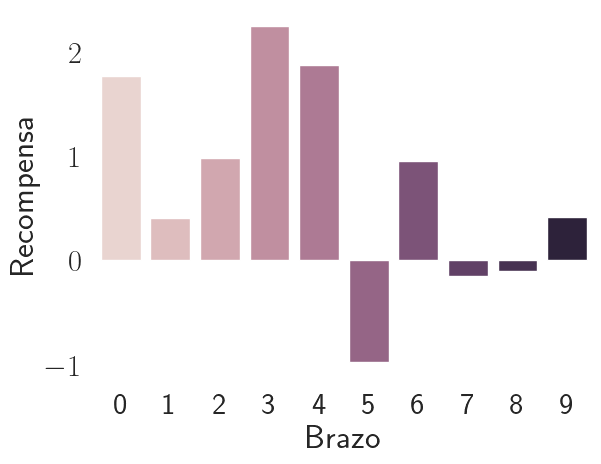
\includegraphics[width=\textwidth]{../img/rewards_sigma_0}
            \caption{$\sigma=0$}
            \label{fig:rewards_0}
        \end{subfigure}
        \begin{subfigure}[H]{0.3\textwidth}
            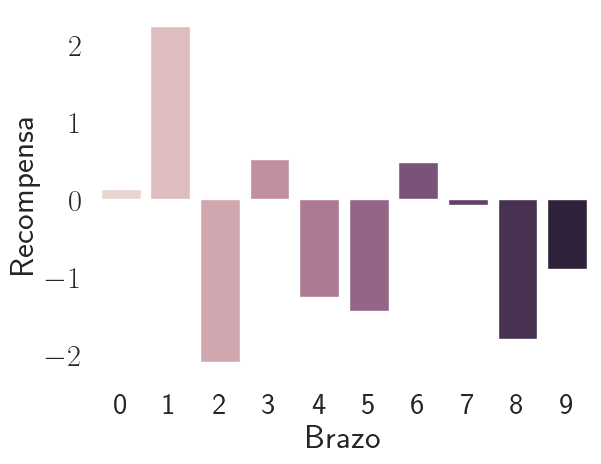
\includegraphics[width=\textwidth]{../img/rewards_sigma_1}
            \caption{$\sigma=1$}
            \label{fig:rewards_1}
        \end{subfigure}
        \begin{subfigure}[H]{0.3\textwidth}
            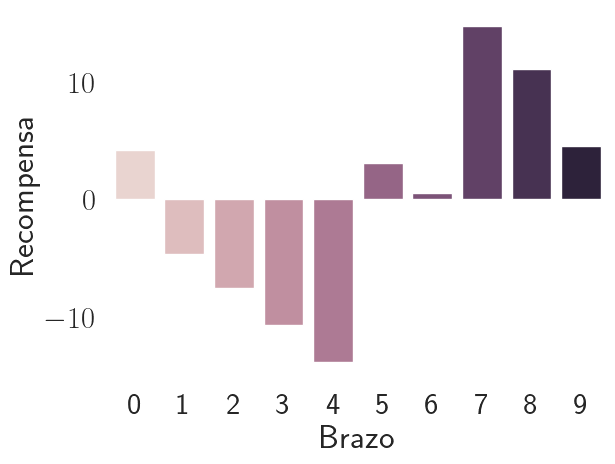
\includegraphics[width=\textwidth]{../img/rewards_sigma_10}
            \caption{$\sigma=10$}
            \label{fig:rewards_10}
        \end{subfigure}
        \caption{Recompensa para cada brazo}
        \label{fig:rewards}
    \end{figure}

    Se aplicó el algoritmo $\varepsilon-greedy$ con distintas combinaciones de $\varepsilon$ y $\sigma$.
    Los resultados de los \textit{Q-valor} de las acciones se muestran en la Figura~\ref{fig:estimations}.

    \begin{figure}[H]
        \centering

        \begin{subfigure}[H]{0.3\textwidth}
            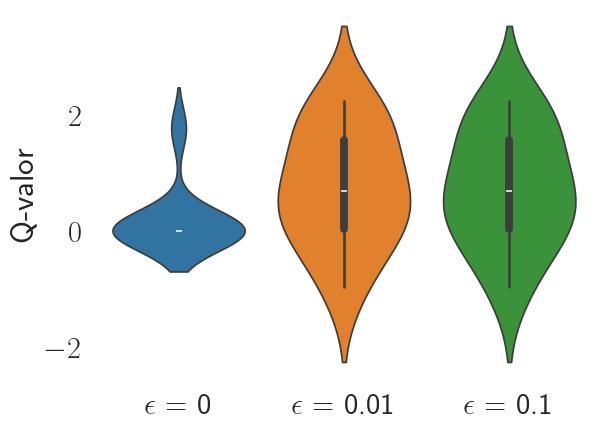
\includegraphics[width=\textwidth]{../img/values_sigma_0}
            \caption{$\sigma=0$}
            \label{fig:estimations_0}
        \end{subfigure}
        \begin{subfigure}[H]{0.3\textwidth}
            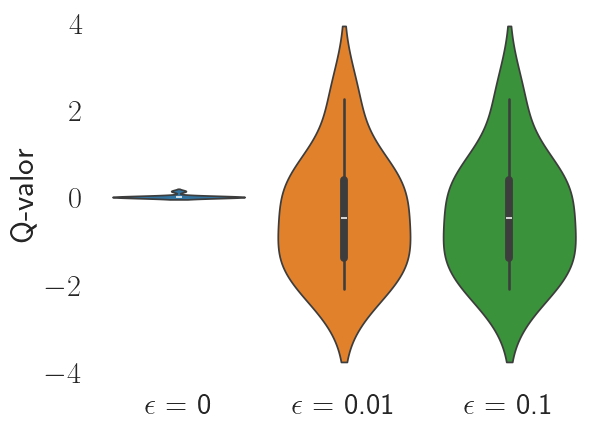
\includegraphics[width=\textwidth]{../img/values_sigma_1}
            \caption{$\sigma=1$}
            \label{fig:estimations_1}
        \end{subfigure}
        \begin{subfigure}[H]{0.3\textwidth}
            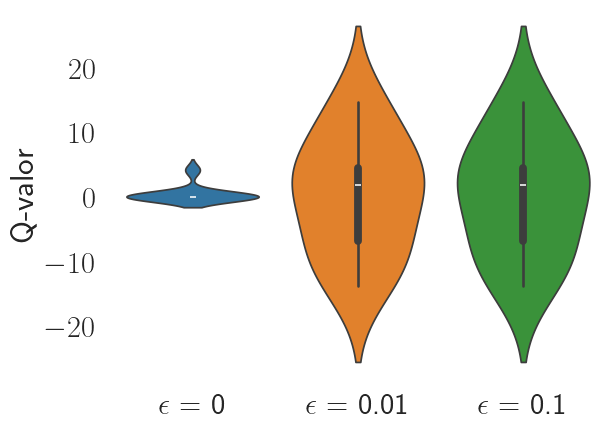
\includegraphics[width=\textwidth]{../img/values_sigma_10}
            \caption{$\sigma=10$}
            \label{fig:estimations_2}
        \end{subfigure}

        \caption{\textit{Q-Valor} de las acciones}
        \label{fig:estimations}
    \end{figure}

    La Figura~\ref{fig:arms_selected} muestra el número de veces que se seleccionó cada brazo para los distintos valores de $\varepsilon$ y $\sigma$.

    \begin{figure}[H]
        \centering
        \begin{subfigure}[H]{0.3\textwidth}
            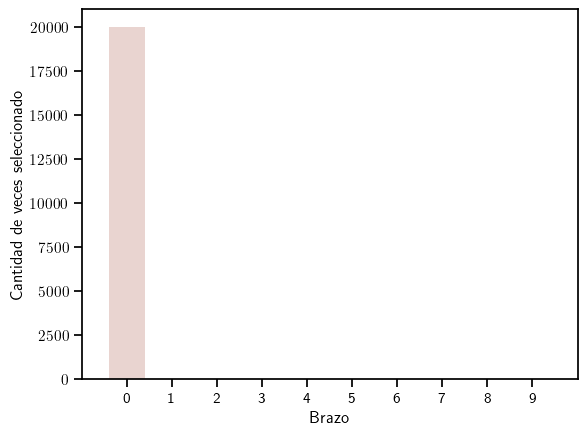
\includegraphics[width=\textwidth]{../img/arm_sigma_0_epsilon_0}
            \caption{$\sigma=0 ,\ \varepsilon=0$}
            \label{fig:arms_selected_0_0}
        \end{subfigure}
        \begin{subfigure}[H]{0.3\textwidth}
            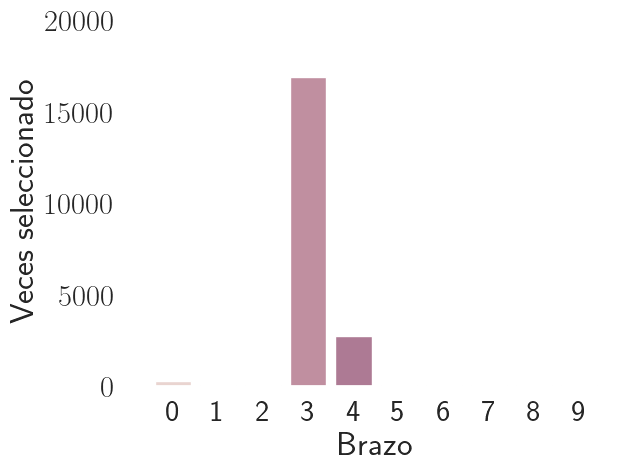
\includegraphics[width=\textwidth]{../img/arm_sigma_0_epsilon_0.01}
            \caption{$\sigma=0 ,\ \varepsilon=0.01$}
            \label{fig:arms_selected_0_0.01}
        \end{subfigure}
        \begin{subfigure}[H]{0.3\textwidth}
            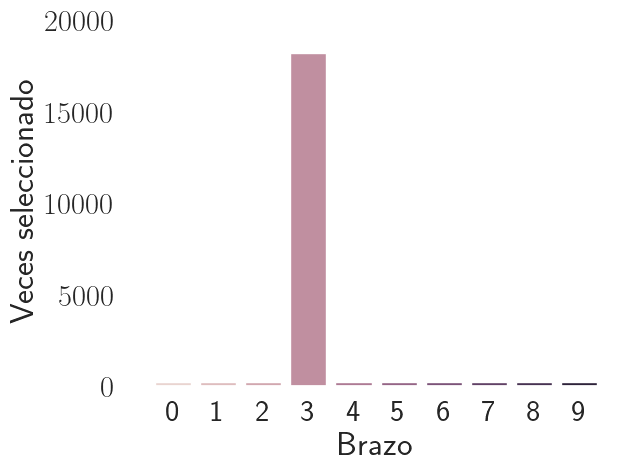
\includegraphics[width=\textwidth]{../img/arm_sigma_0_epsilon_0.1}
            \caption{$\sigma=0 ,\ \varepsilon=0.10$}
            \label{fig:arms_selected_0_0.1}
        \end{subfigure}

        \begin{subfigure}[H]{0.3\textwidth}
            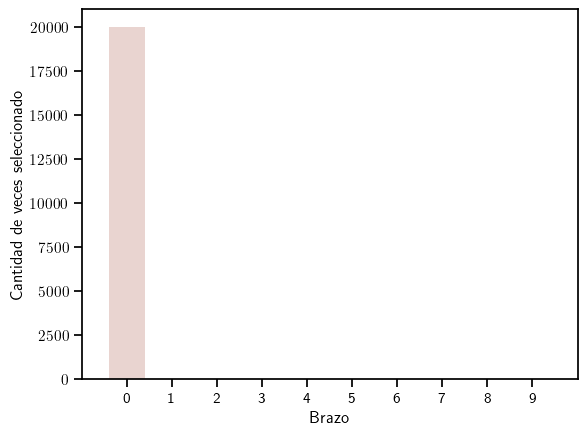
\includegraphics[width=\textwidth]{../img/arm_sigma_1_epsilon_0}
            \caption{$\sigma=1 ,\ \varepsilon=0$}
            \label{fig:arms_selected_1_0}
        \end{subfigure}
        \begin{subfigure}[H]{0.3\textwidth}
            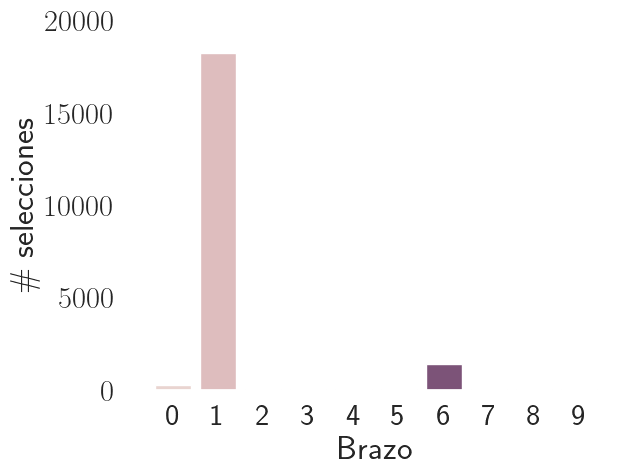
\includegraphics[width=\textwidth]{../img/arm_sigma_1_epsilon_0.01}
            \caption{$\sigma=1 ,\ \varepsilon=0.01$}
            \label{fig:arms_selected_1_0.01}
        \end{subfigure}
        \begin{subfigure}[H]{0.3\textwidth}
            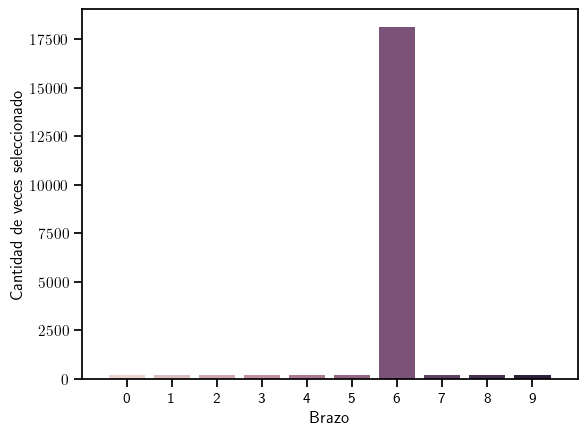
\includegraphics[width=\textwidth]{../img/arm_sigma_1_epsilon_0.1}
            \caption{$\sigma=1 ,\ \varepsilon=0.10$}
            \label{fig:arms_selected_1_0.1}
        \end{subfigure}

        \begin{subfigure}[H]{0.3\textwidth}
            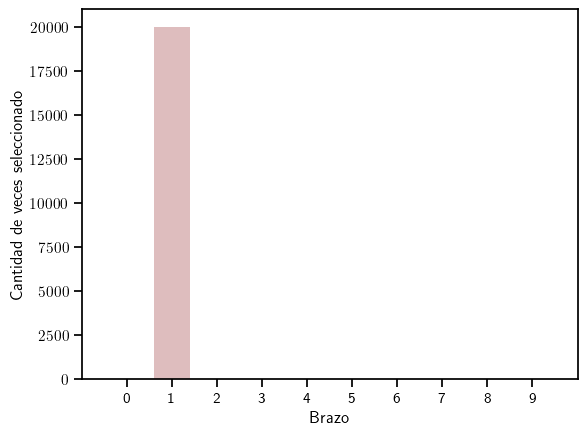
\includegraphics[width=\textwidth]{../img/arm_sigma_10_epsilon_0}
            \caption{$\sigma=10 ,\ \varepsilon=0$}
            \label{fig:arms_selected_10_0}
        \end{subfigure}
        \begin{subfigure}[H]{0.3\textwidth}
            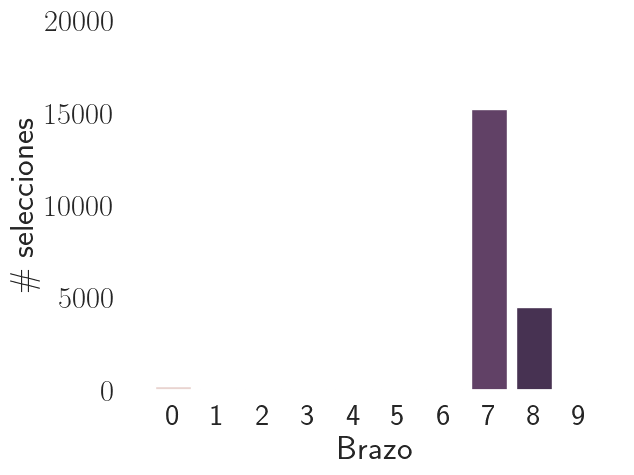
\includegraphics[width=\textwidth]{../img/arm_sigma_10_epsilon_0.01}
            \caption{$\sigma=10 ,\ \varepsilon=0.01$}
            \label{fig:arms_selected_10_0.01}
        \end{subfigure}
        \begin{subfigure}[H]{0.3\textwidth}
            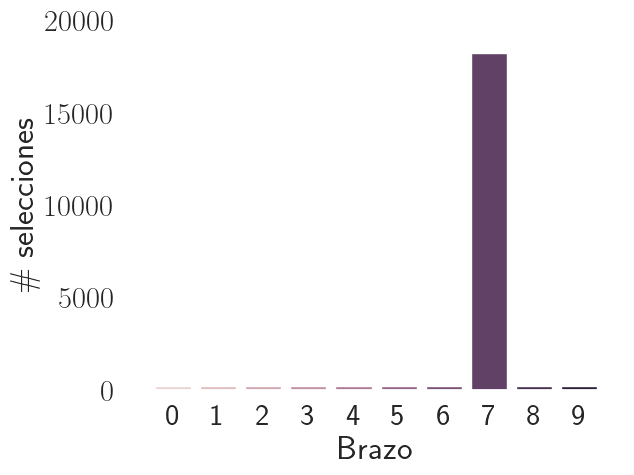
\includegraphics[width=\textwidth]{../img/arm_sigma_10_epsilon_0.1}
            \caption{$\sigma=10 ,\ \varepsilon=0.10$}
            \label{fig:arms_selected_10_0.1}
        \end{subfigure}

        \caption{Número de veces que se seleccionó cada brazo}
        \label{fig:arms_selected}
    \end{figure}

    Finalmente, se analizó la recompensa promedio obtenida en función del número de iteraciones para los distintos valores de $\varepsilon$ y $\sigma$.
    Los resultados se muestran en la Figura~\ref{fig:average_reward}.

    \begin{figure}[H]
        \centering
        \begin{subfigure}[H]{0.3\textwidth}
            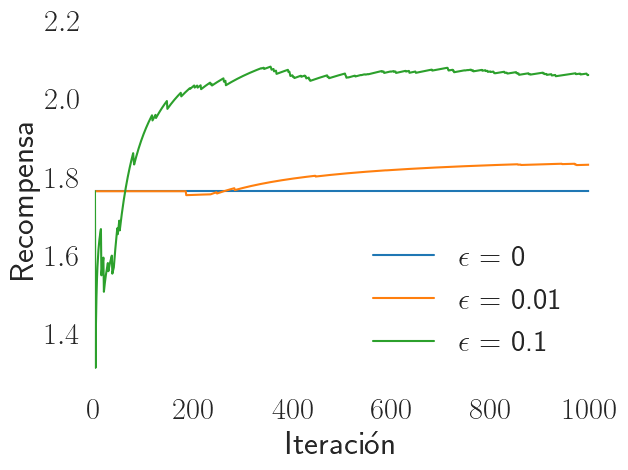
\includegraphics[width=\textwidth]{../img/reward_iteration_sigma_0}
            \caption{$\sigma=0$}
            \label{fig:average_reward_0}
        \end{subfigure}
        \begin{subfigure}[H]{0.3\textwidth}
            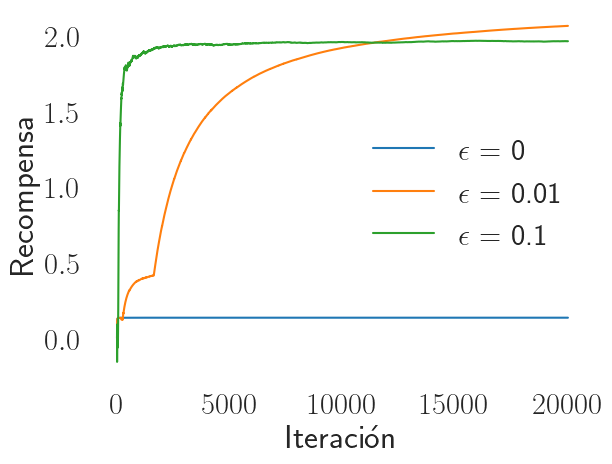
\includegraphics[width=\textwidth]{../img/reward_iteration_sigma_1}
            \caption{$\sigma=1$}
            \label{fig:average_reward_1}
        \end{subfigure}
        \begin{subfigure}[H]{0.3\textwidth}
            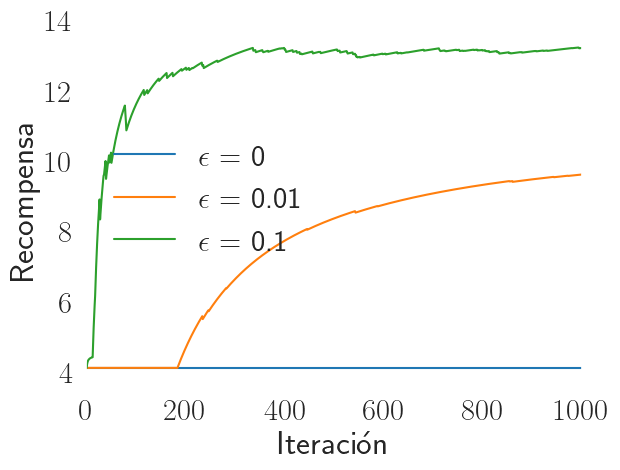
\includegraphics[width=\textwidth]{../img/reward_iteration_sigma_10}
            \caption{$\sigma=10$}
            \label{fig:average_reward_10}
        \end{subfigure}
        \caption{Recompensa promedio obtenida}
        \label{fig:average_reward}
    \end{figure}

    \underline{\textbf{Conclusiones}}\\
    \textbf{Efecto de $\varepsilon$}:\\

    \begin{itemize}
        \item \textbf{$\varepsilon=0$}: El algoritmo se comporta como un método de explotación pura, eligiendo siempre la acción con la mejor recompensa estimada.
        Esto puede llevar a un rendimiento subóptimo si la estimación inicial es incorrecta.
        \item \textbf{$\varepsilon=0.01$ y $\varepsilon=0.10$}: Se observó una mejora en la exploración de acciones no elegidas previamente, lo que permitió al algoritmo encontrar mejores acciones a largo plazo.
        Un mayor valor de ε (como 0.10) permitió una exploración más agresiva, lo que resultó en un rendimiento más equilibrado.
        ε (como 0.10) permitió una exploración más agresiva, lo que resultó en un rendimiento más equilibrado.

%    Fomenta que el algoritmo explore más y no explota las acciones que han demostrado ser más prometedoras.
%    En todos los casos, según la Figura~\ref{fig:average_reward}, $\varepsilon=0.01$ obtiene la mayor recompensa cuando $n \rightarrow \infty$.
%    Para el caso de $\varepsilon=0.0$ y $\varepsilon=0.10$, la recompensa promedio se mantuvo constante y no se observó una mejora significativa en la recompensa promedio obtenida cuando $n \rightarrow \infty$, a diferencia de $\varepsilon=0.01$ cuyas recompensas crecen más despacio al inicio, pero supera a las otras dos opciones a medida que $n$ aumenta.

    \textbf{Efecto de $\sigma$}: A medida que el desvío estándar $\sigma$ aumenta, la recompensa promedio obtenida disminuye.
    Esto se debe a que las recompensas son más inciertas y, por lo tanto, es más difícil para el algoritmo encontrar la acción óptima.

    \textbf{Interacción entre $\varepsilon$ y $\sigma$}: Para $\sigma=0$, el algoritmo converge rápidamente a la acción óptima, independientemente de $\varepsilon$.
    Sin embargo, para $\sigma=1$ y $\sigma=10$, el algoritmo converge más lentamente y la elección de $\varepsilon$ puede afectar significativamente la recompensa promedio obtenida.

    \textbf{Exploración vs. Explotación}: La elección de $\varepsilon$ afecta la exploración y explotación del algoritmo.

    \textbf{Desempeño del algoritmo}: El desempeño del algoritmo depende de la interacción entre $\varepsilon$ y $\sigma$.

    \begin{itemize}

        \item

        \item
        \item
        \item
        \item \textbf{Optimización de $\varepsilon$}: La elección de $\varepsilon$ depende de la naturaleza del problema y de la importancia de la exploración y explotación.
        \item \textbf{Optimización de $\sigma$}: La elección de $\sigma$ depende de la incertidumbre de las recompensas y de la importancia de la precisión en la estimación de los valores de las acciones.
        \item \textbf{Balance entre exploración y explotación}: En general, es importante encontrar un balance entre la exploración y la explotación para maximizar la recompensa promedio obtenida.
    \end{itemize}

    \line(1,0){\textwidth}

    \indent\underline{\textbf{Ejercicio 6}}\\
    Dada la fórmula adaptativa del valor $Q_{n+1}= Q_n+\alpha\left[R_{n}-Q_{n}\right]$ con $\alpha\in\left(0,1\right]$, demostrar que

    \begin{itemize}
        \item $Q_{n+1}=(1-\alpha)^{n}Q_{n} + \sum_{i=1}^n \alpha(1-\alpha)^{n-i}R_{i}$
        \item $(1-\alpha)^{n}+\sum_{i=1}^{n} \alpha(1-\alpha)^{n-i}=1$, es decir, $Q_{n+1}$ es un promedio pesado de $Q_{n},R_1,R_2,\dots,R_n$.
    \end{itemize}

    \indent\underline{\textbf{Solución}}\\

    Sea,\\
    $Q_{n}$: Valor estimado de la acción después de haber sido seleccionada $n-1$ veces \\
    $R_i$: Recompensa obtenida después de la $i$-ésima selección de la acción \\
    $n$: Número de veces que la acción ha sido seleccionada \\
    $\alpha\in\left(0,1\right]$: \textit{step-size} constante \\
    $Q_{n+1}$: Valor estimado de la acción después de haber sido seleccionada $n$ veces \\

    \textbf{Primera parte}\\
    La fórmula adaptativa para calcular el valor $Q_{n+1}$ se puede expresar como

    \begin{align*}
        Q_{n+1} &= Q_n+\alpha\left[R_{n}-Q_{n}\right] \\
        &= Q_n + \left(1-\alpha\right)Q_n + \alpha R_n
    \end{align*}

    Si $n=1$,

    \[
        Q_{2} = \left(1-\alpha\right)Q_1 + \alpha R_1
    \]

    Si $n=2$,

    \[
        Q_{3} = \left(1-\alpha\right)Q_2 + \alpha R_2
    \]

    Lo que coincide con la fórmula en cuestión,

    \begin{align*}
        Q_{2} &= (1-\alpha)^{1}Q_{1} + \sum_{i=1}^{1} \alpha(1-\alpha)^{1-i}R_{i} \\
        Q_{2}&= (1-\alpha)Q_{1} + \alpha R_{1} \\
        & \ldots \ldots \ldots \\
        Q_{3} &= (1-\alpha)^{2}Q_{2} + \sum_{i=1}^{2} \alpha(1-\alpha)^{2-i}R_{i} \\
        Q_{3}& = (1-\alpha)^{2}Q_{2} + \alpha(1-\alpha)R_{1} + \alpha R_{2}
    \end{align*}

    Si se generaliza para $n$, se tiene que

    \begin{align*}
        Q_{n+1} &= (1-\alpha)^{n}Q_{n} + \sum_{i=1}^{n} \alpha(1-\alpha)^{n-i}R_{i} \\
        &= (1-\alpha)^{n}Q_{n} + \alpha(1-\alpha)^{n-1}R_{1} + \alpha(1-\alpha)^{n-2}R_{2} + \ldots + \alpha R_{n}
    \end{align*}

    \textbf{Segunda parte}\\
    Se desea demostrar que $(1-\alpha)^{n}+\sum_{i=1}^{n} \alpha(1-\alpha)^{n-i}=1$.
    La expresión se puede reescribir como

    \[
        \sum_{i=1}^{n} \alpha\left( 1 - \alpha \right)^{n-i} = \alpha\sum_{i=1}^{n} \left( 1 - \alpha \right)^{n-i}
    \]

    Se sustituye $j=n-i$, tal que cuando $i=1$, $j=n-1$ y cuando $i=n$, $j=0$.

    \[
        \sum_{j=0}^{n-1} \left( 1-\alpha \right)^{j}
    \]

    El último término de la expresión anterior es la suma de una serie geométrica, la cual se puede expresar como

    \[
        \sum_{j=0}^{n-1} \left( 1-\alpha \right)^{j} = \frac{1-(1-\alpha)^n}{\alpha}
    \]

    Al sustituir $(1-\alpha)^n + \alpha \left( \frac{1-(1-\alpha)^n}{\alpha} \right)$ en la expresión original, se obtiene

    \[
        (1-\alpha)^n + \frac{1-(1-\alpha)^n}{\alpha} = 1
    \]

    Esto implica que $Q_{n+1}$ es un promedio pesado de los valores $Q_{n},R_1,R_2,\dots,R_n$, donde los pesos están determinados por los términos de la serie geométrica.

    \line(1,0){\textwidth}

    \indent\underline{\textbf{Ejercicio 7}}\\
    Demostrar que fórmula adaptativa para calcular el valor $Q_{n+1}=Q_n+\alpha\left[R_n-Q_n\right]$ con  \textit{step-size} $\alpha\in\left(0,1\right]$ constante no verifica las hipótesis del teorema de convergencia y, por lo tanto, no está garantizada su convergencia.

    \indent\underline{\textbf{Solución}}\\
    La fórmula adaptativa para calcular el valor $Q_{n+1}$ se puede expresar como

    \[
        Q_{n+1} = (1-\alpha)Q_n + \alpha R_n
    \]

    Es decir, el valor de $Q_{n+1}$ es una combinación lineal de los valores anteriores $Q_n$ y la recompensa $R_n$.

    \textbf{Análisis de convergencia}\\
    Para que la secuencia $Q_n$ converja se deben cumplir las condiciones:

    \begin{itemize}
        \item \textbf{Condición de convergencia}: El \textit{step-size} $\alpha$ debe decrecer a lo largo del tiempo, es decir, $\alpha_n \rightarrow 0$ cuando $n \rightarrow \infty$.
        \item \textbf{Acotamiento}: La secuencia $Q_n$ debe estar acotada, es decir, $Q_n$ debe estar acotada para todo $n$.
    \end{itemize}

    El caso en cuestión plantea que $\alpha$ es constante, es decir, $\alpha_n = \alpha,\ \forall n$.
    Por lo tanto, el término $R_n - Q_n$ no se reduce a lo largo del tiempo, lo que impide que la secuencia $Q_n$ converja, o bien, su valor presente oscilaciones.

    En conclusión, teniendo en cuenta los teoremas sobre convergencia de sucesiones:

    \begin{itemize}
        \item Si el término general no tiende a cero, la secuencia $Q_n$ no converge.
        \item El caso en cuestión, con $\alpha \in (0,1]$, es contante y no decrece.
    \end{itemize}

    Por lo tanto, no se garantiza la convergencia de la secuencia $Q_n$.

    \line(1,0){\textwidth}

    \indent\underline{\textbf{Ejercicio 8}}\\
    En la \textit{Figura 2.3} del libro \textit{Sutton\&Barto (2018)}, se observa un \textit{spike} en el paso número 11 cuando se utiliza inicialización optimista.
    De una explicación de este fenómeno.

    \begin{figure}[H]
        \centering
        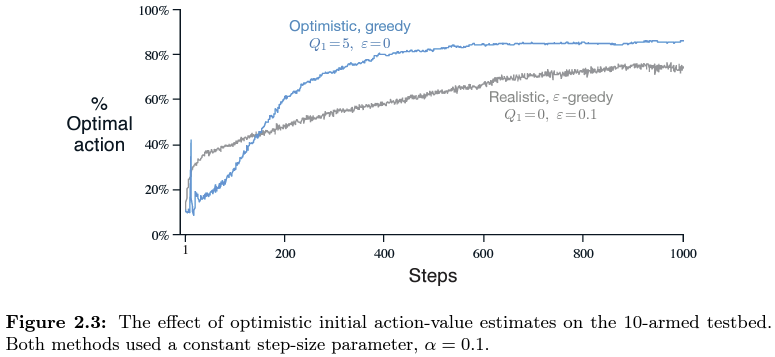
\includegraphics[width=0.5\textwidth]{../img/Figura2_3_SuttonBarto}
        \caption{Figura 2.3 - Sutton\&Barto (2018)}
        \label{fig:fig_2_3}
    \end{figure}

    \indent\underline{\textbf{Solución}}\\
    Sea,\\
    \textbf{Inicialización optimista}: Al inicio de cada episodio, se inicializan los valores de las acciones con un valor alto, por lo que el agente tenderá a probar todas las acciones.
    Esta inicialización fomenta/induce a la exploración.\\
    \textbf{Inicialización realista}: Los valores de las acciones se inicializan con un valor realista, como si no se tuviera información previa sobre las recompensas esperadas.
    Esta inicialización fomenta/induce a la explotación.\\

    El spike en cuestión se debe a la inicialización optimista de los valores de las acciones.
    Al corresponder a valores altos, el agente tenderá a probar todas las acciones, lo que puede llevar a obtener recompensas altas en los primeros pasos.
    En otras palabras, el agente lleva a cabo una búsqueda más agresiva al inicio del episodio.

    \line(1,0){\textwidth}

    \indent\underline{\textbf{Ejercicio 9}}\\
    Demuestre que la función \textit{SOFTMAX}: $p(a)=\frac{e^{H(a)}}{\sum_{a'=1}^{K} e^{H(a')}}$, define una distribución de probabilidades discreta válida.

    \indent\underline{\textbf{Solución}}\\
    Para demostrar que la función SOFTMAX define una distribución de probabilidades discreta válida, se deben cumplir las siguientes condiciones:

    \textbf{No negatividad}\\
    La probabilidad de cada acción debe ser no negativa, es decir, $p(a) \geq 0$.
    Es decir,

    \[
        p(a) = \frac{e^{H(a)}}{\sum_{a'=1}^{K} e^{H(a')}} \geq 0, \quad \forall a
    \]

    Notar que,

    \begin{itemize}
        \item \textbf{Numerador}: $e^{H(a)} \geq 0$, ya que $e^{x} > 0$ para todo $x$.
        \item \textbf{Denominador}: $\sum_{a'=1}^{K} e^{H(a')} > 0$, ya que es la suma de los valores exponenciales de las acciones.
        \item \textbf{División}: La división de dos valores positivos es positiva.
    \end{itemize}

    Por lo tanto, la probabilidad de cada acción es no negativa, es decir, $p(a) \geq 0$.

    \textbf{Suma unitaria}\\
    La suma de las probabilidades de todas las acciones debe ser igual a uno, es decir, $\sum_{a=1}^{K} p(a) = 1$.

    Para tal efecto se demuestra que la suma de las probabilidades de todas las acciones es igual a uno.

    \[
        \sum_{a=1}^{K} p(a) = 1
    \]

    O bien,

    \[
        \sum_{a=1}^{K} \frac{e^{H(a)}}{\sum_{a'=1}^{K} e^{H(a')}} = 1
    \]

    El cociente puede expresarse como,

    \[
        \frac{1}{\sum_{a'=1}^{K} e^{H(a')}} \sum_{a=1}^{K} e^{H(a)} = 1
    \]

    La suma de los valores exponenciales de las acciones es igual a la suma de los valores exponenciales de las acciones, lo que implica que la suma de las probabilidades de todas las acciones es igual a uno.
    En otras palabras, la suma en el numerador es igual a la suma en el denominador.

    \begin{align*}
        \frac{ \sum_{a=1}^{K} e^{H(a)} } {\sum_{a'=1}^{K} e^{H(a')}} &= 1 \\
        \sum_{a=1}^{K} p(a) = \frac{ \sum_{a=1}^{K} e^{H(a)} } {\sum_{a'=1}^{K} e^{H(a')}} &= 1\\
        \sum_{a=1}^{K} p(a) &= 1
    \end{align*}

    Se concluye que la función \textit{SOFTMAX} define una distribución de probabilidades discreta válida.

    \line(1,0){\textwidth}

    \indent\underline{\textbf{Ejercicio 10}}\\
    Demostrar que las derivadas de la función SOFTMAX $p(x)$ respecto de sus parámetros $H(a),\ a=1,2,\dots,K$, son iguales a:

    \[
        \frac{\partial p(x)}{\partial H(a)} =
        \begin{cases}
            p(x)(1-p(x))    &\text{si $x = a$} \\
            -p(x)p(a)       &\text{si $x\neq a$}
        \end{cases}
    \]

    \indent\underline{\textbf{Solución}}\\
    Se calcula la derivada cuando $a=b$

    \[
        \frac{\partial p(a)}{\partial H(a)} = \frac{\partial}{\partial H(a)} \left( \frac{e^{H(a)}}{\sum_{a'=1}^{K} e^{H(a')}} \right)
    \]

    Se sustituyó $Z=\sum_{a'=1}^{K} e^{H(a')}$ previamente,

    \begin{align*}
        \frac{\partial p(a)}{\partial H(a)} &= \frac{\partial}{\partial H(a)} \left( \frac{e^{H(a)}}{Z} \right) \\
        &= \frac{Z\cdot e^{H(a)} - e^{H(a)}\cdot \frac{\partial Z}{\partial H(a)}}{Z^2} \\
    \end{align*}

    Se calcula la derivada de $Z$ respecto de $H(a)$, es decir, $\frac{\partial Z}{\partial H(a)}$

    \begin{align*}
        Z &= \sum_{a'=1}^{K} e^{H(a')} \\
        \frac{\partial Z}{\partial H(a)} &= e^{H(a)}
    \end{align*}

    Se sustituye en la expresión anterior,

    \begin{align*}
        \frac{\partial p(a)}{\partial H(a)} &= \frac{Z\cdot e^{H(a)} - e^{H(a)}\cdot e^{H(a)}}{Z^2} \\
        &= \frac{Z\cdot e^{H(a)} - e^{2H(a)}}{Z^2} \\
        &= \frac{e^{H(a)}(Z - e^{H(a)})}{Z^2}
    \end{align*}

    Además, $p(a) = \frac{e^{H(a)}}{Z}$, por lo que

    \begin{align*}
        Z &= p(a) + \sum_{b\neq a} e^{H(b)} \\
        &= p(a) + (1-p(a))Z
    \end{align*}

    Por lo tanto,
    \[
        Z - e^{H(a)} = (1-p(a))Z = (1-p(x))Z
    \]

    Finalmente,

    \[
        \frac{\partial p(a)}{\partial H(a)} = p(x)(1-p(x))
    \]

    Se calcula la derivada cuando $a\neq b$.
    Sea,

    \[
        p(b) = \frac{e^{H(b)}}{Z}
    \]

    Se calcula la derivada de $p(b)$ respecto de $H(a)$,

    \begin{align*}
        \frac{\partial p(b)}{\partial H(a)} &= 0 -0 + (-1) \cdot Z^{-2} \cdot e^{H(b)} \cdot e^{H(a)} \\
        &= -p(b)p(x)
    \end{align*}

    Se concluye que las derivadas de la función SOFTMAX $p(x)$ respecto de sus parámetros $H(a),\ a=1,2,\dots,K$, son iguales a:

    \[
        \frac{\partial p(x)}{\partial H(a)} =
        \begin{cases}
            p(x)(1-p(x))    &\text{si $x = a$} \\
            -p(x)p(a)       &\text{si $x\neq a$}
        \end{cases}
    \]

    \line(1,0){\textwidth}

    \indent\underline{\textbf{Ejercicio 11}}\\
    Demostrar que la regla de actualización por gradiente ascendente estocástico:

    \[
        H_{t+1}(a) = H_t (a) + \alpha \frac{\partial E[R_t] }{\partial H_t(a)},
    \]

    con $E[R_t] = \sum_{x=1}^{K} p_t(x)q_{*}(x)$, puede escribirse de la siguiente manera:

    \[
        H_{t+1}(a) =
        \begin{cases}
            H_t (a) + \alpha (R_t - C)(1-p_t(a))    &\text{si $a = A_t$} \\
            H_t (a) - \alpha (R_t - C)p_t(a)        &\text{si $a \neq A_t$}
        \end{cases}
    \]

    \indent\underline{\textbf{Solución}}\\
    Se calcula la derivada de $E[R_t]$ respecto de $H_t(a)$,

    \begin{align*}
        \frac{\partial E[R_t]}{\partial H_t(a)} &= \sum_{x=1}^{K} q_{*}(x) \frac{\partial p_t(x)}{\partial H_t(a)}
    \end{align*}

    Además, $p_t(x) = \frac{e^{H_t(x)}}{\sum_{x'=1}^{K} e^{H_t(x')}}$, por lo que si $x=a$,

    \begin{align*}
        \frac{\partial p_t(x)}{\partial H_t(a)} &= p_t(x)(1-p_t(x))
    \end{align*}

    Si $x\neq a$,

    \begin{align*}
        \frac{\partial p_t(x)}{\partial H_t(a)} &= -p_t(x)p_t(a)
    \end{align*}

    Por lo tanto, si $a=A_t$ la derivada de $E[R_t]$ respecto de $H_t(a)$ es

    \begin{align*}
        \frac{\partial E[R_t]}{\partial H_t(a)} &= q_{*}(a)p_t(a)(1-p_t(a)) + \sum_{x\neq a} q_{*}(x)(-p_t(b)p_t(a)) \\
        &= p(a)\left( q_{*}(a)(1-p_t(a)) - \sum_{x\neq a} q_{*}(x)p_t(a) \right) \\
    \end{align*}

    El término entre paréntesis es igual a $R_t - C$, siendo $C$ el costo esperado,

    \[
        C = E[R_t] = \sum_{x=1}^{K} p_t(x)q_{*}(x)
    \]

    Al sustituir en la expresión anterior, se obtiene

    \[
        \frac{\partial E[R_t]}{\partial H_t(a)} = p(a)(R_t - C)
    \]

    Lo anterior es válido para $R=q_{*}(A)$, es decir, la recompensa esperada es igual a la recompensa óptima.

    Por lo tanto, tras remplazar en la regla de actualización por gradiente ascendente estocástico, se obtiene

    \[
        H_{t+1}(a) =
        \begin{cases}
            H_t (a) + \alpha (R_t - C)(1-p_t(a))    &\text{si $a = A_t$} \\
            H_t (a) - \alpha (R_t - C)p_t(a)        &\text{si $a \neq A_t$}
        \end{cases}
    \]


    \line(1,0){\textwidth}

%    \paragraph{Referencias}\label{par:references}
%    \lipsum[5]
%
%    \paragraph{Apéndice}\label{par:appendix}
%
%    \lipsum[5]


\end{document}
